\section{Understanding Non-Stationarity in MARL}\label{sec:background-non-stationarity}
In MARL, when the policies of all other agents in the environment are stationary, they can be considered to be effectively a part of the environment from the perspective of each agent, resulting in a stationary single agent Markov decision process for each agent to learn from. 
However, in practice, the other agents in the environment are not fixed, but rather always learning from their recent experiences. As we detail in this section, this results in the inherent non-stationarity of MARL because Markovian update functions for each agent induce a Markov chain of joint policies. Indeed, when the policies of other agents constantly change, the problem is effectively non-stationary from each agent's perspective if the other agents are viewed as part of the environment.  
%The combination of an MDP and fixed policy for each agent naturally induces a Markov chain of states. 
%We can formally understand the inherent non-stationarity of MARL by considering the Markov chain of joint policies induced . 
%We start by explaining a general multiagent framework based on a stochastic game between $n$ agents and then introduce how a set of Markovian policy update rules for each agent inherently induces the non-stationarity problem.
% This perspective results in our key observation that the sequential dependencies between a meta-agent's current policy and the other agents' future policies exist in a general multiagent learning problem, which is a key insight behind Meta-MAPG. 
% as the peer agents are also learning agents based on trajectories by interacting with a meta-agent (please refer to Figure 1b)
% The combination of 1) an MDP 2) a set of policies for each agent and 3) a set of markovian update rules for each agent induces a markov chain in the joint parameter space.

\subsection{Stochastic Games}
Interactions between multiple agents can be represented by stochastic games~\citep{shapley53stochastic}. 
Specifically, an $n$-agent stochastic game is defined as a tuple $\mathcal{M}_{n}\!=\!\langle \mathbfcal{I}, \mathbfcal{S}, \mathbfcal{A}, \mathcal{P}, \mathbfcal{R}, \gamma \rangle$;
$\mathbfcal{I}\!=\!\{1,\sdots,n\}$ is the set of $n$ agents, 
$\mathbfcal{S}$ is the set of states, 
$\mathbfcal{A}\!=\!\times_{i \in \mathcal{I}} \mathcal{A}^{i}$ is the set of action spaces, 
$\mathcal{P}\!:\!\mathbfcal{S}\times\mathbfcal{A}\mapsto \mathbfcal{S}$ is the state transition probability function,
$\mathbfcal{R}\!=\!\times_{i \in \mathcal{I}} \mathcal{R}^{i}$ is the set of reward functions, and
$\gamma\!\in\![0,1)$ is the discount factor.
We typeset sets in bold for clarity.
Each agent $i$ executes an action at each timestep $t$ according to its stochastic policy $a^i_t\!\sim\!\pi^{i}(a^{i}_{t}|s_{t},\phi^i)$ parameterized by $\phi^{i}$, where $s_{t}\!\in\!\mathbfcal{S}$.
A joint action $\bm{a}_{\bm{t}}\!=\!\{a^{i}_t,\bm{a}^{\bm{-i}}_{\bm{t}}\}$ yields a transition from the current state $s_{t}$ to the next state $s_{t+1}\!\in\!\mathbfcal{S}$ with probability $\mathcal{P}(s_{t+1}|s_t,\bm{a}_{\bm{t}})$, where the notation $\bm{-i}$ indicates all other agents with the exception of agent $i$.
Agent $i$ then obtains a reward according to its reward function $r^{i}_t\!=\!\mathcal{R}^i(s_t,\bm{a}_{\bm{t}})$.
At the end of an episode, the agents collect a trajectory $\tau_{\bm{\phi}}$ under the joint policy with parameters $\bm{\phi}$, where $\tau_{\bm{\phi}}\!:=\!(s_{0},\bm{a}_{\bm{0}},\bm{r}_{\bm{0}},\sdots,\bm{r}_{\bm{H}})$, $\bm{\phi}\!=\!\{\phi^{i},\bm{\phi}^{\bm{-i}}\}$ represents the joint parameters of all policies, $\bm{r}_{\bm{t}}\!=\!\{r^{i}_{t},\bm{r}^{\bm{-i}}_{\bm{t}}\}$ is the joint reward, and $H$ is the episode horizon.

%%%%%%%%%%%%%%%%%%%%%%%%%%%%%%%%%%%%%%%%%%%%%%%%%%%%%%%%%%%%%%%%%%%%%%%%%%%%%%%%%
\begin{figure}[t]
   \captionsetup[subfigure]{skip=0pt, aboveskip=2pt}
   \begin{subfigure}[b]{\linewidth}
        \centering
        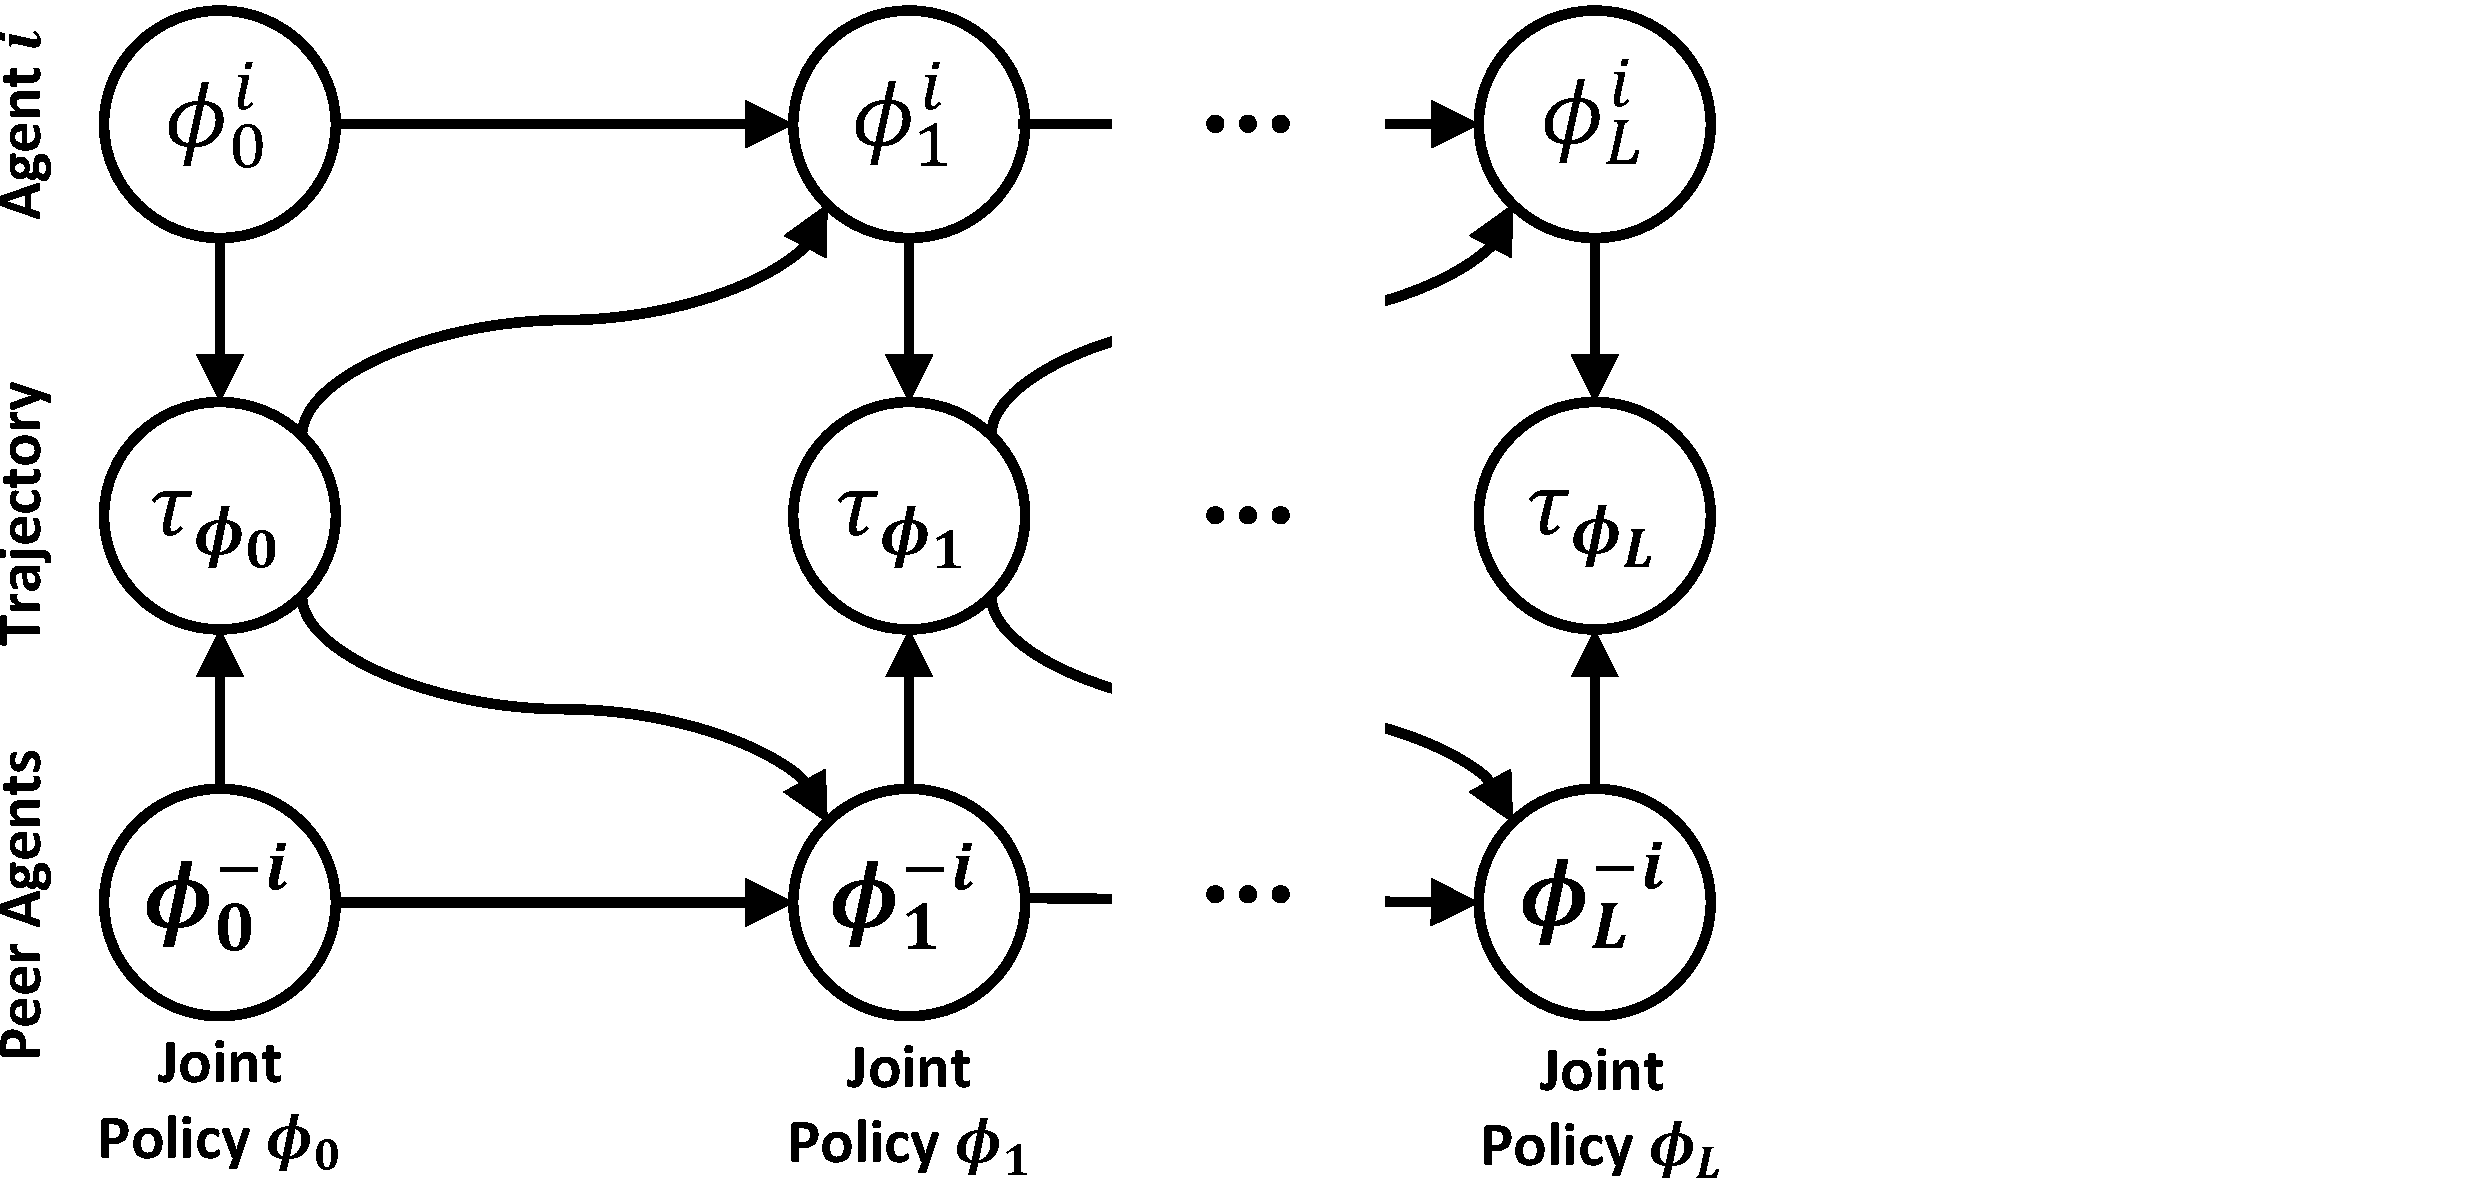
\includegraphics[height=3.1cm]{figs/markov_chain.pdf}
        \caption{}
        \label{fig:markov-chain}
    \end{subfigure}
    \begin{subfigure}[b]{\linewidth}
        \centering
        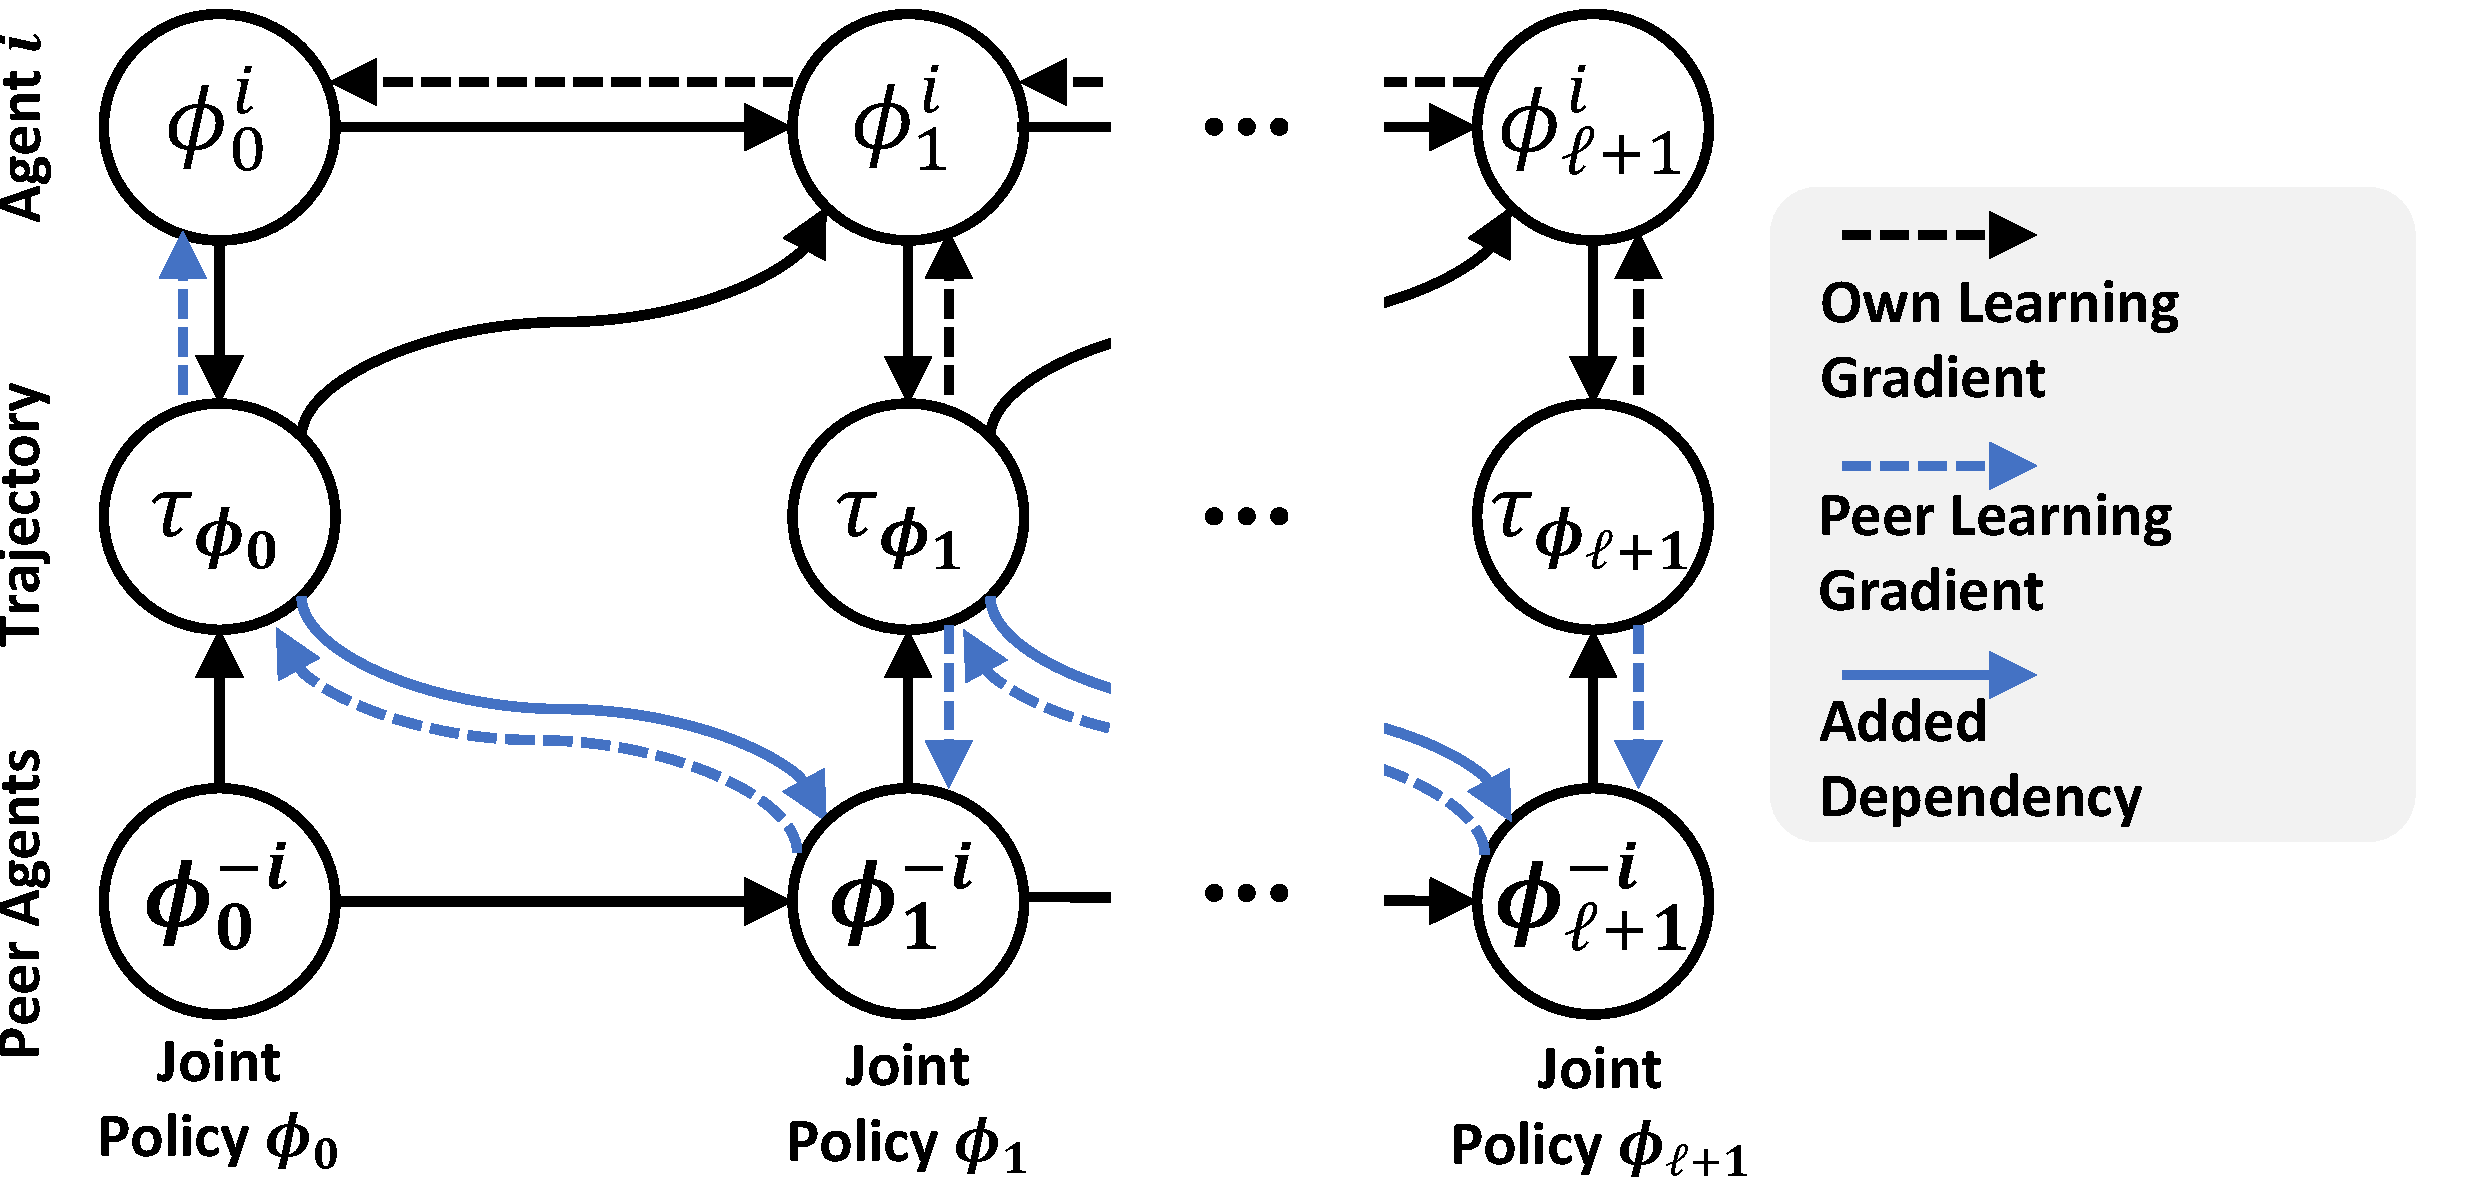
\includegraphics[height=3.1cm]{figs/meta_mapg.pdf}
        \caption{}
        \label{fig:graph-meta-mapg}
    \end{subfigure}
    \vspace{-0.8cm}
    \caption{
        \textbf{(a)} A Markov chain of joint policies representing the inherent non-stationarity of MARL. Each agent updates its policy leveraging a Markovian update function, resulting in a change to the joint policy. 
        \textbf{(b)} A probabilistic graph for Meta-MAPG. Unlike Meta-PG, our approach actively influences the future policies of other agents as well through the peer learning gradient.
        }
    \vskip-0.18in
\end{figure}
%%%%%%%%%%%%%%%%%%%%%%%%%%%%%%%%%%%%%%%%%%%%%%%%%%%%%%%%%%%%%%%%%%%%%%%%%%%%%%%%%

\subsection{A Markov Chain of Joint Policies}\label{sec:markov-chain-of-policies}
% While the underlying multiagent environment can be stationary, the perceived non-stationarity in multiagent settings results from a 
The perceived non-stationarity in multiagent settings results from a distribution of sequential joint policies, which can be represented by a Markov chain.
Formally, a Markov chain of policies begins from a stochastic game between agents with an initial set of joint policies parameterized by $\bm{\phi}_{\bm{0}}\!=\!\{\phi^{i}_{0},\bm{\phi}^{\bm{-i}}_{\bm{0}}\}$. 
We assume that each agent updates its policy leveraging a Markovian update function $\phi^{i}_{1}\!\sim\!U^{i}(\tau_{\bm{\phi}_{\bm{0}}},\phi^{i}_{0})$ that changes the policy after every $K$ trajectories. 
After this time period, each agent $i$ updates its policy in order to maximize the expected return expressed as its value function:%~\citep{Sutton:1998}:
% \begin{align}\label{eqn:value-function}
% \begin{split}
% V^{i}_{\bm{\phi}_{\bm{0}}}(s_{0})&=\mathbb{E}_{p(\tau_{\bm{\phi}_{\bm{0}}}|\bm{\phi}_{\bm{0}})}\Big[\smallsum_{t=0}^{H}\gamma^{t}r^{i}_{t}|s_{0}\Big]\\&=\mathbb{E}_{p(\tau_{\bm{\phi}_{\bm{0}}}|\bm{\phi}_{\bm{0}})}\Big[G^{i}(\tau_{\bm{\phi}_{\bm{0}}})\Big],
% \end{split}
% \end{align}
\begin{gather}
\!\!\!V^{i}_{\!\bm{\phi}_{\bm{0}}}\!(s_{0})\!=\!\mathbb{E}_{p(\tau_{\bm{\phi}_{\bm{0}}}\!|\bm{\phi}_{\bm{0}})}\!\Big[\!\smallsum_{t=0}^{H}\!\!\gamma^{t}r^{i}_{t}|s_{0}\hspace{-0.1em}\Big]\!\!=\!\mathbb{E}_{p(\tau_{\bm{\phi}_{\bm{0}}}\!|\bm{\phi}_{\bm{0}})}\!\Big[\!G^{i}(\tau_{\!\bm{\phi}_{\bm{0}}})\!\Big]\!,\label{eqn:value-function}
\end{gather}
% \begin{gather}
% V^{i}_{\bm{\phi}_{\bm{0}}}(s_{0})\!=\!\mathbb{E}_{p(\tau_{\bm{\phi}_{\bm{0}}}\!|\bm{\phi}_{\bm{0}})}\Big[\smallsum_{t=0}^{H}\!\gamma^{t}r^{i}_{t}|s_{0}\Big]\!=\!\mathbb{E}_{p(\tau_{\bm{\phi}_{\bm{0}}}\!|\bm{\phi}_{\bm{0}})}\Big[G^{i}(\tau_{\bm{\phi}_{\bm{0}}})\Big]\!,\nonumber
% \end{gather}
where $G^{i}$ denotes agent $i$'s discounted return from the beginning of an episode with initial state $s_0$.
The joint policy update results in a transition from $\bm{\phi}_{\bm{0}}$ to the updated set of joint parameters $\bm{\phi}_{\bm{1}}$.
The Markov chain continues for a maximum chain length of $L$ (see~\cref{fig:markov-chain}). 
This Markov chain perspective highlights the following inherent aspects of the experienced non-stationarity:

\begin{enumerate}[leftmargin=*, wide, labelindent=0pt, topsep=0pt, label=\arabic*)]
    \itemsep0em 
    \item \textbf{Sequential dependency:} The future joint policy parameters $\bm{\phi}_{\bm{1:L}}\!=\!\{\bm{\phi}_{\bm{1}}, \sdots,\bm{\phi}_{\bm{L}}\}$ sequentially depend on $\bm{\phi}_{\bm{0}}$ since a change in $\tau_{\bm{\phi}_{\bm{0}}}$ results in a change in $\bm{\phi}_{\bm{1}}$, which in turn affects $\tau_{\bm{\phi}_{\bm{1}}}$ and all successive joint policy updates up to $\bm{\phi}_{\bm{L}}$. 
    \item\textbf{Controllable levels of non-stationarity:} As in~\citet{alshedivat2018continuous} and~\citet{foerster17lola}, we assume stationary policies during the collection of $K$ trajectories, and that the joint policy update happens afterward. In such a setting, it is possible to control the non-stationarity by adjusting the $K$ and $H$ hyperparameters: smaller $K$ and $H$ increase the rate that agents change their policies, leading to a higher degree of non-stationarity in the environment.
\end{enumerate}